\section{Data Cleaning and Processing}
This section details the steps undertaken to prepare the dataset for training and testing the Cassava Leaf Disease Classification model. The dataset was analyzed, cleaned, and processed to ensure proper training and evaluation. 

\subsection{\textbf{Exploratory Data Analysis (EDA)}}
The dataset initially contained 21,397 images categorized into five classes. Analysis of the training dataset revealed the following class distribution shown in Figure~\ref{fig:ImbalancedData}.

\begin{figure}[t]
    \centering
    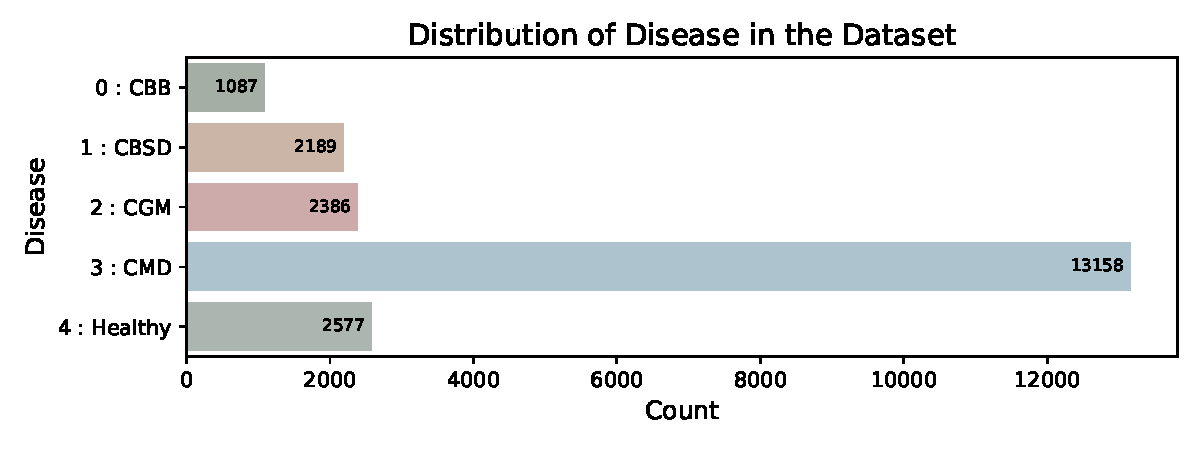
\includegraphics[width=1\linewidth]{graphs/overview/Distribution of Disease in the Dataset.pdf}
    \caption{Imbalanced Cassava Disease Label Distribution}
    \label{fig:ImbalancedData}
\end{figure}

Figure~\ref{fig:ImbalancedData} highlighted a significant class imbalance, with Label 3 accounting for over 60\% of the dataset, while Label 0 represented only 5\%. To address this imbalance and explore its impact on the model’s performance, two dataset preparation strategies were employed: Balanced Data and Imbalanced Data with Train-Validation Split.

\subsection{\textbf{Dataset Preparation }}
\subsubsection{Balancing the Data}

To address the class imbalance in the training dataset, a validation set of 500 samples was created by randomly sampling 100 images from each class.
The remaining samples were allocated to the training set, resulting in the new distribution shown in Figure~\ref{fig:BalancedDataset}.

\begin{itemize}
    \item \textbf{Train Set:} 20,897 samples.
    \item \textbf{Validation Set:} 500 samples.
    \item \textbf{Test Set:} 1 sample (reserved for evaluation consistency).
\end{itemize}

\begin{figure}[t]
    \centering
    \begin{subfigure}{0.4\textwidth}
        \centering
        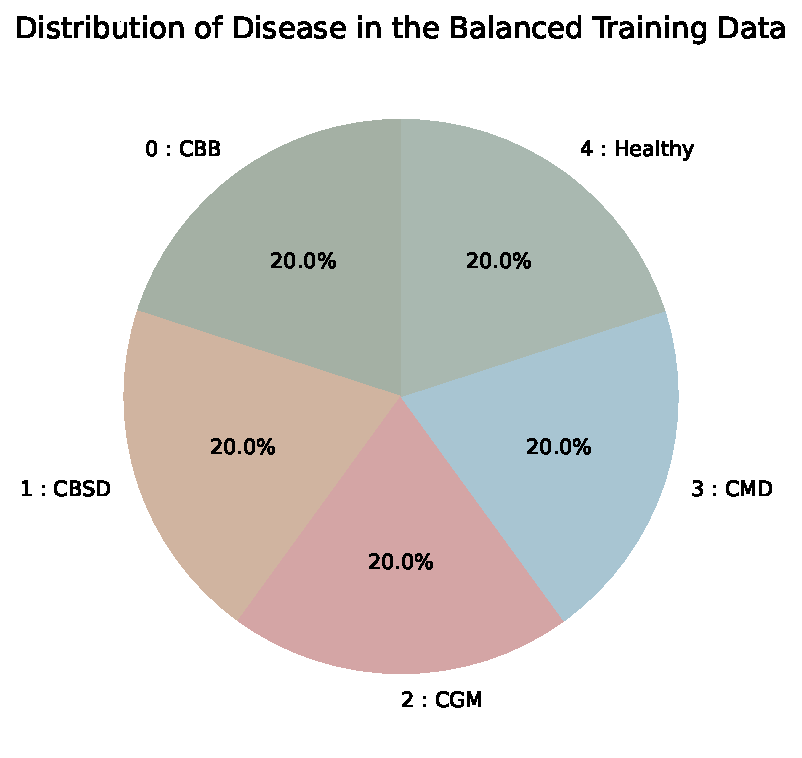
\includegraphics[width=\linewidth]{graphs/overview/Distribution of Disease in the Balanced Training Data.pdf}
        \caption{Balanced Train Dataset}
        \label{fig:BalancedTrain}
    \end{subfigure}
    \begin{subfigure}{0.4\textwidth}
        \centering
        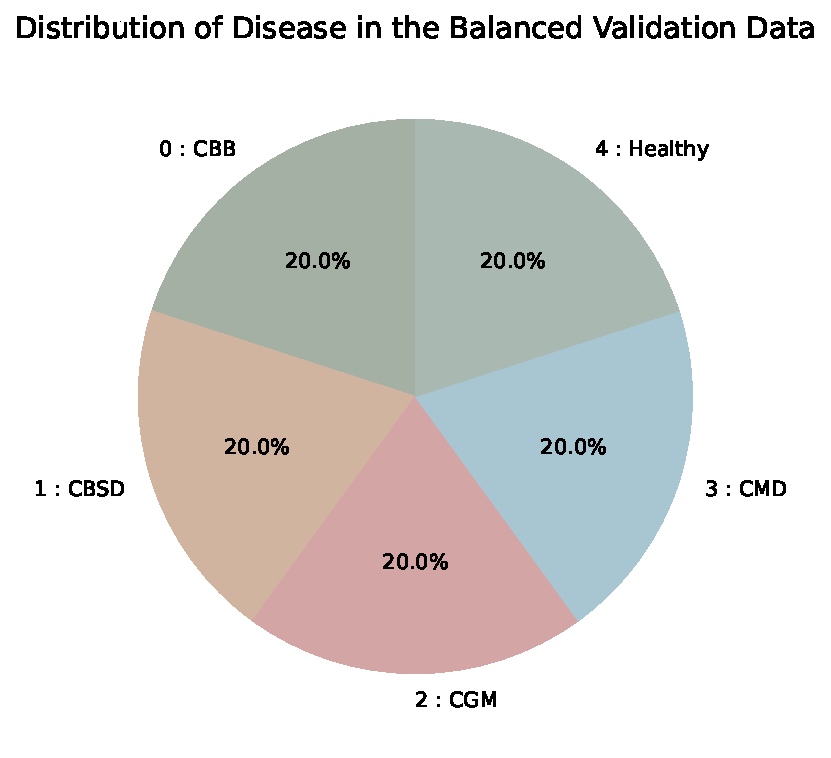
\includegraphics[width=\linewidth]{graphs/overview/Distribution of Disease in the Balanced Validation Data.pdf}
        \caption{Balanced Val Dataset}
        \label{fig:BalancedVal}
    \end{subfigure}
    \caption{Balanced Cassava Disease Label Distribution}
    \label{fig:BalancedDataset}
\end{figure} 

The training data was further balanced by down-sampling all classes to the size of the smallest class (\textbf{987 samples}). This ensured an equal representation of all classes as seen in Figure[\ref{fig:BalancedDataset}]

By addressing the imbalance, this approach aims to ensure that the model receives equal exposure to all classes during training. This is particularly beneficial for smaller classes that might otherwise be under-represented.

\subsubsection{Train-Validation Split with Imbalanced Data}
To maintain the original class distribution, a separate train-validation split was performed without balancing the dataset:

\begin{itemize}
    \item \textbf{Train Set:} 95\% of the dataset (\textbf{20,327 samples}).
    \item \textbf{Validation Set:} 5\% of the dataset (\textbf{1,070 samples}).
    \item \textbf{Test Set:} 1 sample.
\end{itemize}

The distribution is described in Figure~\ref{fig:TrainValSplit}. This split allows the model to learn from the imbalanced distribution, simulating a real-world scenario where imbalances exist. Maintaining the imbalance is essential to evaluate how the model performs without any balancing techniques applied.


\begin{figure}[t]
    \centering
    \begin{subfigure}{0.4\textwidth}
        \centering
        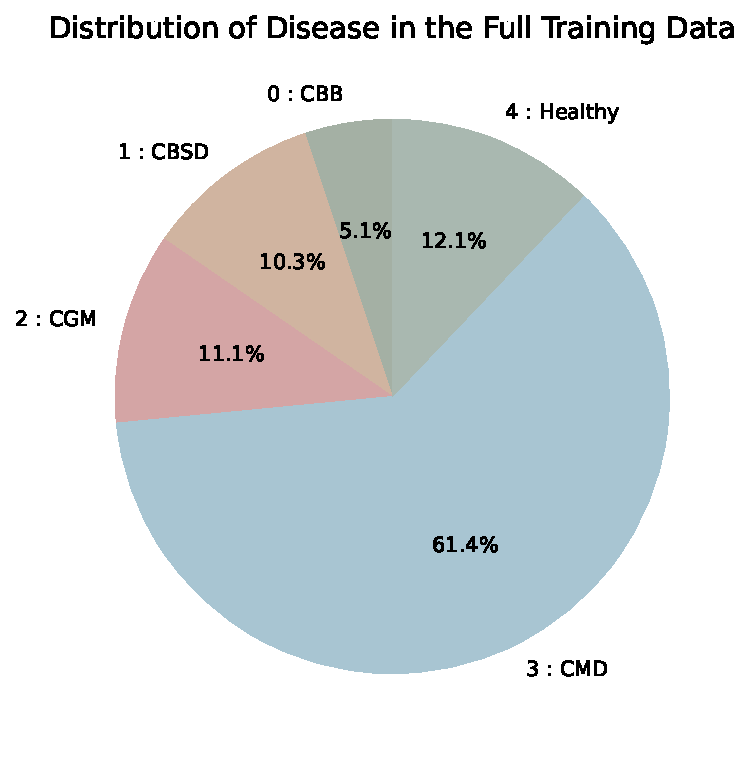
\includegraphics[width=\linewidth]{graphs/overview/Distribution of Disease in the Full Training Data.pdf}
        \caption{Train Dataset 95\%}
        \label{fig:ImbalancedTrain}
    \end{subfigure}
    \begin{subfigure}{0.4\textwidth}
        \centering
        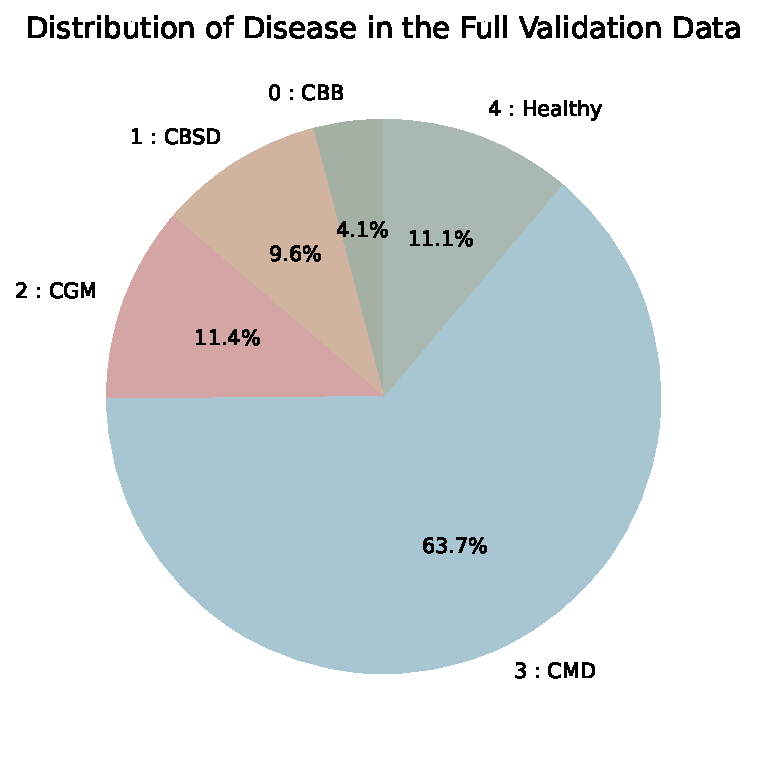
\includegraphics[width=\linewidth]{graphs/overview/Distribution of Disease in the Full Validation Data.pdf}
        \caption{Val Dataset 5\%}
        \label{fig:ImbalancedVal}
    \end{subfigure}
    \caption{Train-Val Split Cassava Disease Label Distribution for the Full Dataset}
    \label{fig:TrainValSplit}
\end{figure} 



\subsection{Data Augmentation}

Data augmentation is a crucial technique in computer vision that is used to enhance the diversity of the training dataset without the need to collect additional data. It helps improve the model's generalization ability by simulating real-world variations, such as changes in orientation, scale, lighting, and color. For this analysis, data augmentation was applied to the training dataset to make the model robust to noise and variations in cassava leaf images.

\subsubsection{Preprocessing Steps for Training}\label{sec:pre_image}
Focused on increasing dataset variability through augmentation (e.g., random rotations, flips, and color jitter) to improve the model's generalization ability and robustness. The detailed reason we do this is described in Section~\ref{sec:overfit}.

The following augmentation techniques were applied during the training phase:

\begin{itemize}
    \item \textbf{Random Rotation:} The images were randomly rotated by up to 45 degrees to account for variations in orientation.
    \item \textbf{Random Resized Crop:} Images were randomly cropped and resized to ensure consistent input size while preserving variability in the content.
    \item \textbf{Random Horizontal Flip:} Horizontal flipping of images was performed to simulate variations in leaf direction.
    \item \textbf{Random Vertical Flip:} Vertical flipping was applied to enhance the diversity of leaf orientations in the training data.
    \item \textbf{Color Jitter:} Random adjustments were made to the brightness, contrast, saturation, and hue of images to account for variations in lighting and color conditions.
    \item \textbf{ToTensor:} The ToTensor transformation was applied to convert the augmented images into PyTorch tensors, ensuring compatibility with deep learning models.
    \item \textbf{Normalization:} Finally, the images were normalized using the mean and standard deviation values obtained from the pretrained image processor. This scales pixel values to a standard range, aiding in faster convergence during training.
\end{itemize}

These transformations were applied during the training phase using the following pipeline:



\begin{lstlisting}
self.train_transforms = Compose(
  [
    RandomRotation(degrees=45),
    RandomResizedCrop(size),
    RandomHorizontalFlip(),
    RandomVerticalFlip(),
    ColorJitter(brightness=0.1, contrast=0.1, saturation=0.1, hue=0.1),
    ToTensor(),
    normalize,
  ]
)
\end{lstlisting}

\begin{figure}[t]
    \centering
    % 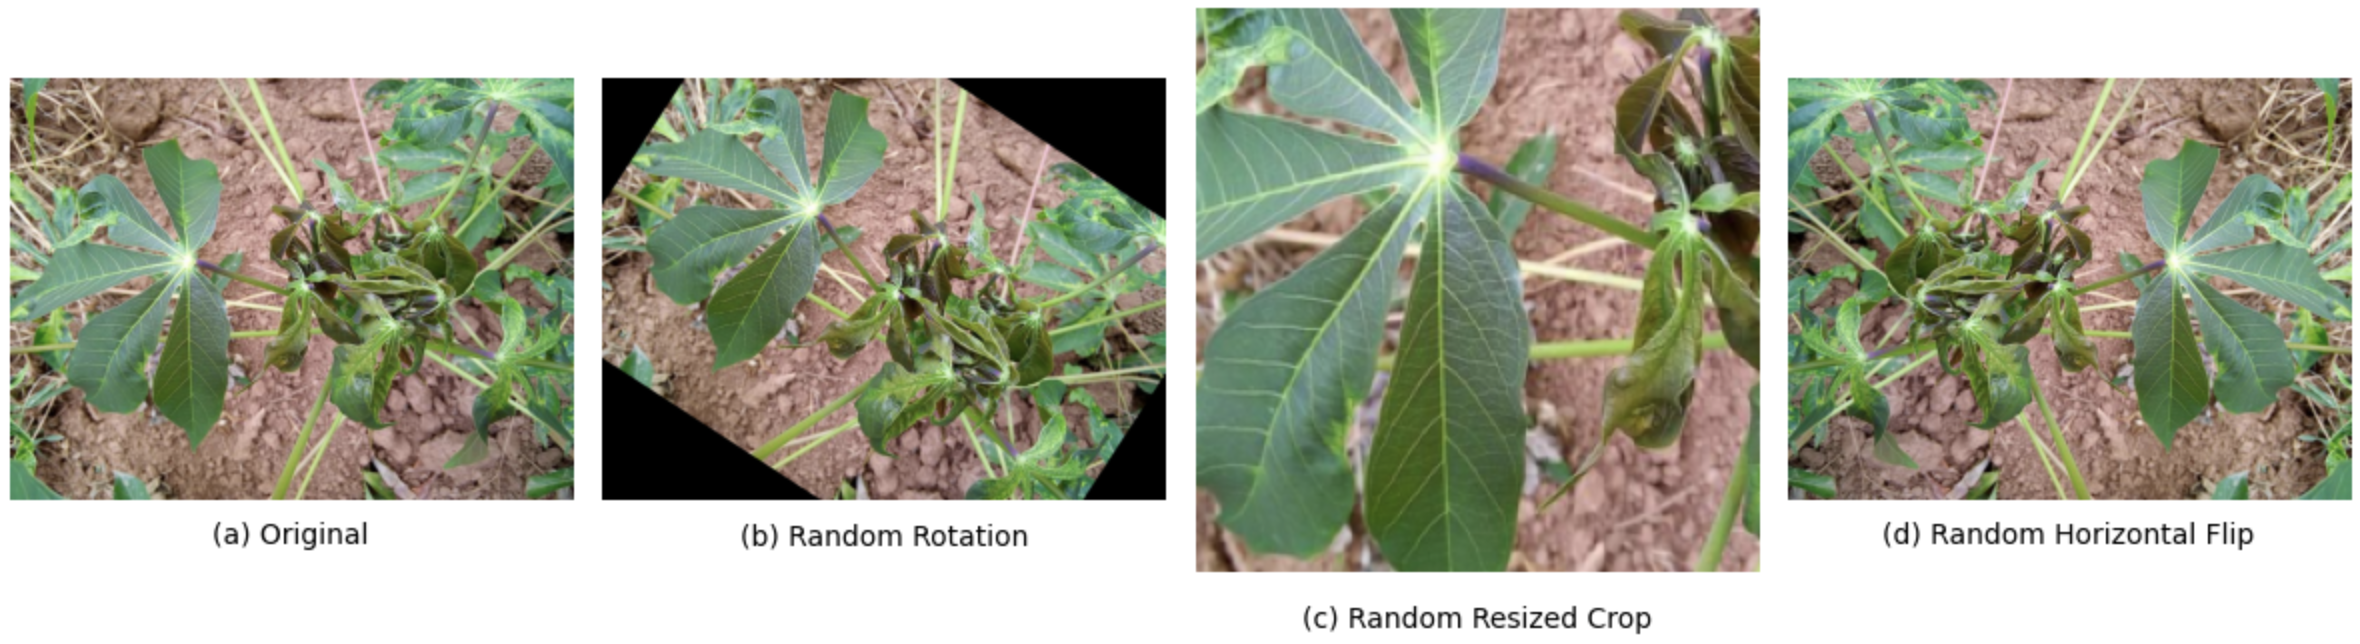
\includegraphics[width=1.0\linewidth]{graphs/TrainDataAug1.png}
    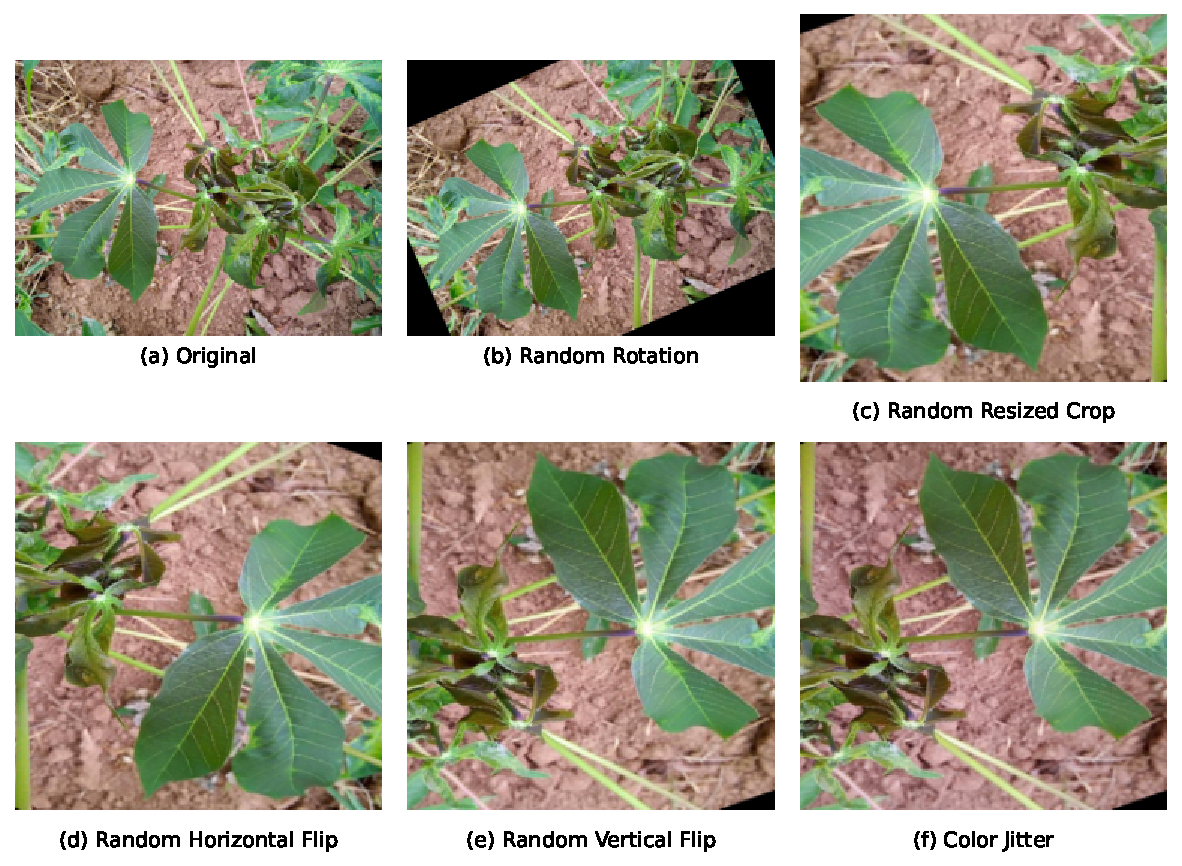
\includegraphics[width=1.0\linewidth]{graphs/overview/TrainTransform.pdf}
    % \centering
    % 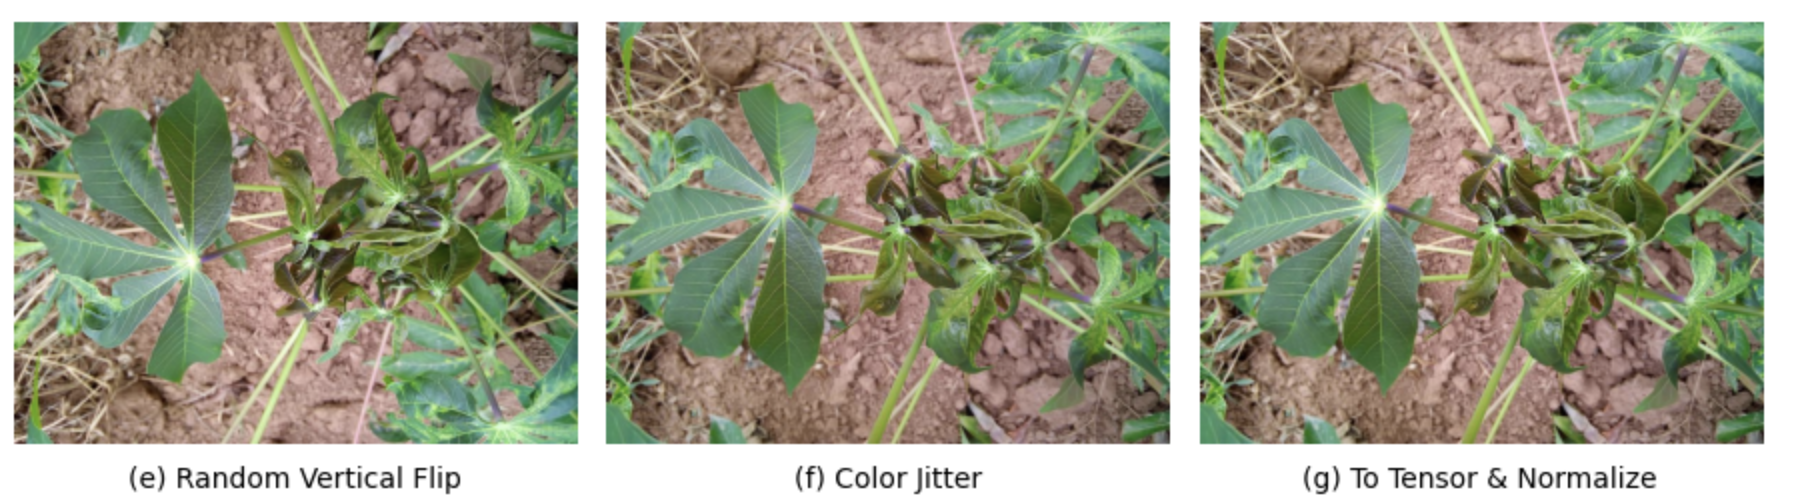
\includegraphics[width=0.8\linewidth]{graphs/TrainDataAug2.png}
    \caption{Data Augmentation on Train Sample}
    \label{fig:TrainAug2}
\end{figure}

To better understand the impact of data augmentation, visualization was performed on the transformations applied to a sample image from the training dataset. Each transformation demonstrates how the training data is modified to improve the model's robustness and generalization as seen in Figure~\ref{fig:TrainAug2}.

\subsubsection{Preprocessing Steps for Validation}

In contrast to the training dataset, the validation dataset underwent simpler preprocessing steps designed to preprocess the images uniformly without augmentation. Although each model has its own image processor, we decided to redefine image processing to ensure the correct order of transformations. This ensures that the evaluation reflects how the model performs on real-world, unaltered images:
\begin{itemize}
    \item \textbf{Resize:} Images were resized to match the input size expected by the model.
    \item \textbf{Center Crop:} A center crop ensured that the main content of the image remained intact while maintaining uniform input dimensions.
    \item \textbf{ToTensor:} Like the training dataset, the validation images were converted into PyTorch tensors to facilitate model compatibility.
    \item \textbf{Normalization:} The same normalization parameters (mean and standard deviation) as used in the training dataset were applied to maintain consistency.
\end{itemize}

For validation, a simpler transformation pipeline was used to standardize the input images:

\begin{lstlisting}
self.val_transforms = Compose(
  [
    Resize(size),
    CenterCrop(size),
    ToTensor(),
    normalize,
  ]
)
\end{lstlisting}

\begin{figure}[t]
    \centering
    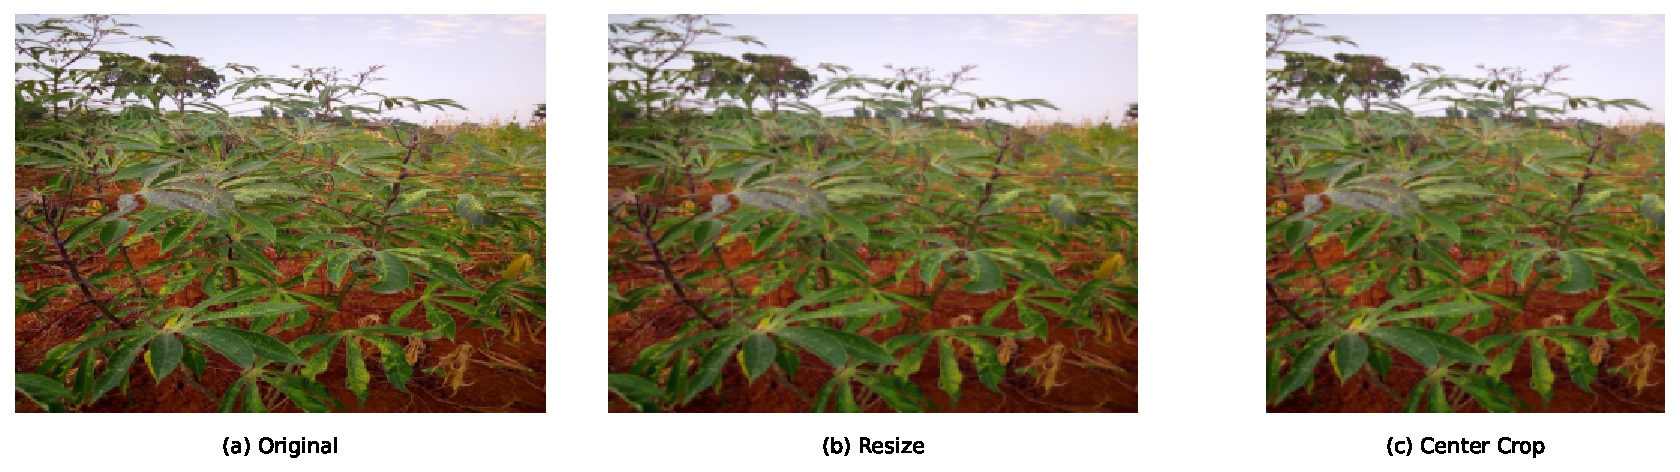
\includegraphics[width=\linewidth]{graphs/overview/ValidationTransform.pdf}
    \caption{Data Augmentation on Val Sample}
    \label{fig:ValDataAug}
\end{figure}

A similar visualization is seen for each step performed in the transformation standardization pipeline for validation data in Figure~\ref{fig:ValDataAug}.

Data augmentation during training enhances the model's ability to generalize, while simpler validation preprocessing ensures consistent and unbiased evaluation of the model's performance. This dual approach strikes a balance between robustness and reliability.

\subsubsection{Further Improvement: Reducing noise with Segment Anything Model}

Most images contain irrelevant background details, such as dirt or leaves from other species, which can introduce localized noise. To address this during preprocessing, we utilize the Segment Anything Model (SAM), an efficient tool for predicting object masks from images and input prompts.

\begin{figure}[H]
    \centering
    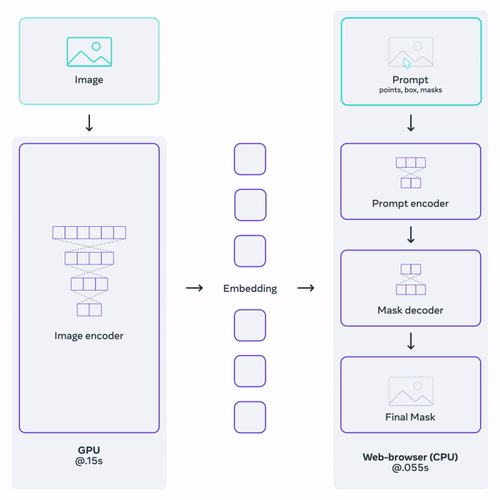
\includegraphics[scale=0.5]{graphs/SAM.jpg}
    \caption{Segment Anything Model Pipeline (Source: Section 3.1c https://segment-anything.com/)}
    \label{fig:SAM}
\end{figure}

Figure \ref{fig:SAM} illustrates how the Segment Anything Model (SAM) operates. SAM uses an image encoder to extract image embeddings and a prompt encoder to process various input prompts, including point coordinates, bounding boxes, and low-resolution masks. The encoded prompts are combined with image embeddings and passed to a mask decoder, which produces the final object masks.

To enable segmentation guided by natural language prompts, we use GroundingDino in conjunction with SAM. GroundingDino is a text-to-bounding-box model that allows users to input an image and a text prompt. It performs zero-shot text-to-bounding-box object detection, effectively identifying objects of interest in an image based on natural language descriptions. The resulting bounding boxes serve as input prompts for SAM, which refines them into accurate segmentation masks.


\begin{figure}[t]
    \centering
    \begin{subfigure}[b]{0.22\linewidth}
        \centering
        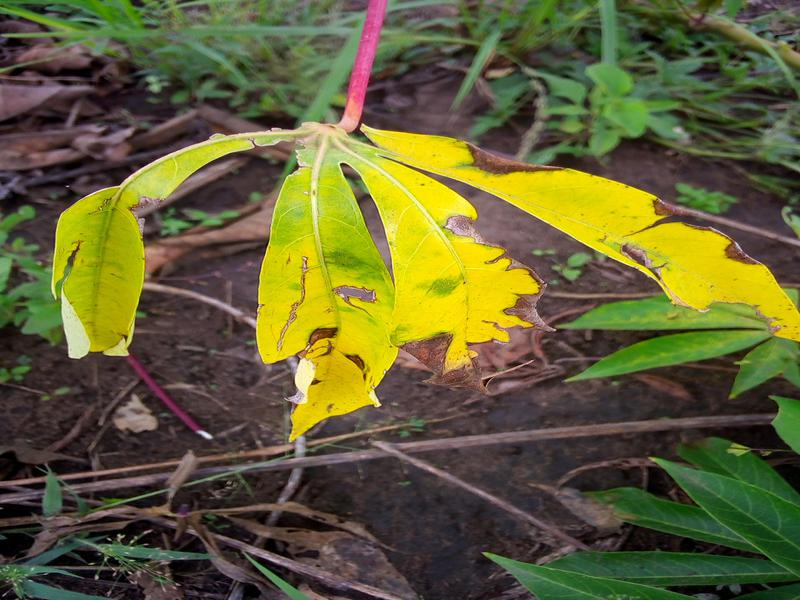
\includegraphics[width=\linewidth]{graphs/samraw1.png}
        \caption{Original Image I}
        \label{fig:Original Image (1)}
    \end{subfigure}
    \hfill
    \begin{subfigure}[b]{0.22\linewidth}
        \centering
        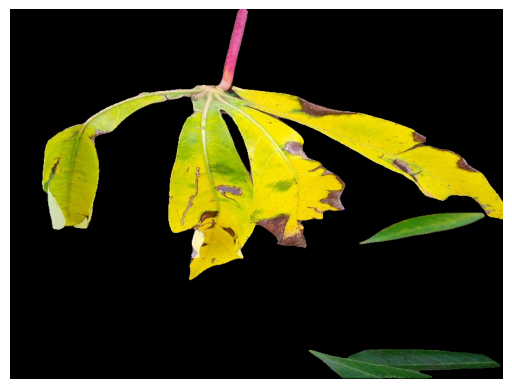
\includegraphics[width=\linewidth]{graphs/sam1.png}
        \caption{Image Mask I}
        \label{fig:Segmentation mask (1)}
    \end{subfigure}
    \hfill
    \begin{subfigure}[b]{0.22\linewidth}
        \centering
        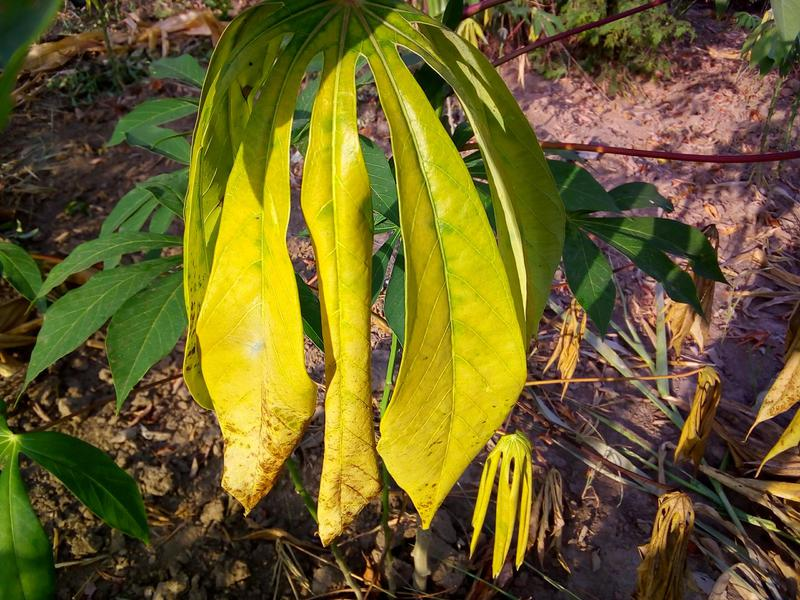
\includegraphics[width=\linewidth]{graphs/samraw2.jpg}
        \caption{Original Image II}
        \label{fig:Original Image (2)}
    \end{subfigure}
     \hfill
     \begin{subfigure}[b]{0.22\linewidth}
        \centering
        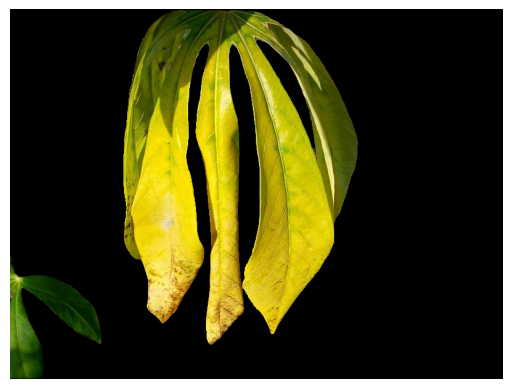
\includegraphics[width=\linewidth]{graphs/sam2.png}
        \caption{Image Mask II}
        \label{fig:Segmentation mask (2)}
    \end{subfigure}
    \caption{Segmentation Masks obtained using Segment Anything Model (SAM)}
    \label{fig:four_images}
\end{figure}

Figure \ref{fig:four_images} illustrates the image before and after processing with SAM. The inverse mask is blacked out to eliminate irrelevant features that contribute to noise. In rare instances where no mask is generated, the entire image is preserved without modifications instead of applying blacking out.